\documentclass[]{article}
\usepackage{lmodern}
\usepackage{amssymb,amsmath}
\usepackage{ifxetex,ifluatex}
\usepackage{fixltx2e} % provides \textsubscript
\ifnum 0\ifxetex 1\fi\ifluatex 1\fi=0 % if pdftex
  \usepackage[T1]{fontenc}
  \usepackage[utf8]{inputenc}
\else % if luatex or xelatex
  \ifxetex
    \usepackage{mathspec}
  \else
    \usepackage{fontspec}
  \fi
  \defaultfontfeatures{Ligatures=TeX,Scale=MatchLowercase}
\fi
% use upquote if available, for straight quotes in verbatim environments
\IfFileExists{upquote.sty}{\usepackage{upquote}}{}
% use microtype if available
\IfFileExists{microtype.sty}{%
\usepackage{microtype}
\UseMicrotypeSet[protrusion]{basicmath} % disable protrusion for tt fonts
}{}
\usepackage[margin=1in]{geometry}
\usepackage{hyperref}
\PassOptionsToPackage{usenames,dvipsnames}{color} % color is loaded by hyperref
\hypersetup{unicode=true,
            pdftitle={Master thesis},
            pdfauthor={Sylvain SCHMITT},
            colorlinks=true,
            linkcolor=Maroon,
            citecolor=Blue,
            urlcolor=Blue,
            breaklinks=true}
\urlstyle{same}  % don't use monospace font for urls
\usepackage{natbib}
\bibliographystyle{plainnat}
\usepackage{longtable,booktabs}
\usepackage{graphicx,grffile}
\makeatletter
\def\maxwidth{\ifdim\Gin@nat@width>\linewidth\linewidth\else\Gin@nat@width\fi}
\def\maxheight{\ifdim\Gin@nat@height>\textheight\textheight\else\Gin@nat@height\fi}
\makeatother
% Scale images if necessary, so that they will not overflow the page
% margins by default, and it is still possible to overwrite the defaults
% using explicit options in \includegraphics[width, height, ...]{}
\setkeys{Gin}{width=\maxwidth,height=\maxheight,keepaspectratio}
\IfFileExists{parskip.sty}{%
\usepackage{parskip}
}{% else
\setlength{\parindent}{0pt}
\setlength{\parskip}{6pt plus 2pt minus 1pt}
}
\setlength{\emergencystretch}{3em}  % prevent overfull lines
\providecommand{\tightlist}{%
  \setlength{\itemsep}{0pt}\setlength{\parskip}{0pt}}
\setcounter{secnumdepth}{5}
% Redefines (sub)paragraphs to behave more like sections
\ifx\paragraph\undefined\else
\let\oldparagraph\paragraph
\renewcommand{\paragraph}[1]{\oldparagraph{#1}\mbox{}}
\fi
\ifx\subparagraph\undefined\else
\let\oldsubparagraph\subparagraph
\renewcommand{\subparagraph}[1]{\oldsubparagraph{#1}\mbox{}}
\fi

%%% Use protect on footnotes to avoid problems with footnotes in titles
\let\rmarkdownfootnote\footnote%
\def\footnote{\protect\rmarkdownfootnote}

%%% Change title format to be more compact
\usepackage{titling}

% Create subtitle command for use in maketitle
\newcommand{\subtitle}[1]{
  \posttitle{
    \begin{center}\large#1\end{center}
    }
}

\setlength{\droptitle}{-2em}
  \title{Master thesis}
  \pretitle{\vspace{\droptitle}\centering\huge}
  \posttitle{\par}
  \author{Sylvain SCHMITT}
  \preauthor{\centering\large\emph}
  \postauthor{\par}
  \predate{\centering\large\emph}
  \postdate{\par}
  \date{2017-05-30}

\usepackage{booktabs}
\usepackage{amsthm}
\makeatletter
\def\thm@space@setup{%
  \thm@preskip=8pt plus 2pt minus 4pt
  \thm@postskip=\thm@preskip
}
\makeatother

\usepackage{amsthm}
\newtheorem{theorem}{Theorem}[section]
\newtheorem{lemma}{Lemma}[section]
\theoremstyle{definition}
\newtheorem{definition}{Definition}[section]
\newtheorem{corollary}{Corollary}[section]
\newtheorem{proposition}{Proposition}[section]
\theoremstyle{definition}
\newtheorem{example}{Example}[section]
\theoremstyle{remark}
\newtheorem*{remark}{Remark}
\begin{document}
\maketitle

\date{}

\thispagestyle{empty}
\begin{center}

\includegraphics{images/main.pdf}
\end{center}

\setlength{\abovedisplayskip}{-5pt}
\setlength{\abovedisplayshortskip}{-5pt}

{
\hypersetup{linkcolor=black}
\setcounter{tocdepth}{2}
\tableofcontents
}
\section*{Résumé et Abstract}\label{resume-et-abstract}
\addcontentsline{toc}{section}{Résumé et Abstract}

Écrire le résumé français ici\ldots{}

Write the english abstract here\ldots{}

\section*{Acknowledgments}\label{acknowledgments}
\addcontentsline{toc}{section}{Acknowledgments}

I would like to thank\ldots{}

\section*{Introduction}\label{introduction}
\addcontentsline{toc}{section}{Introduction}

Sutainable forest management in the tropics (i.e.~managed selective
harvesting of timber) has been widely promoted internationnaly to combat
tropical deforestation and degradation \citep{Zimmerman2012}. Currently
tropical logging accounts for one eight of global timber production
\citep{Blaser2011} and is still increasing. Most tropical timber
production originates from selective logging, the targeted harvesting of
timber from commercial species in a single cuttint cycle
\citep{Martin2015}.

On the other hand, tropical rainforests have fascinated ecologists due
to their outstanding diversity \citep{connell_diversity_1978}.
Effectively tropical forests host over half of the Earth's biodiversity
\citep{Scheffers2012}. High biodiversity from tropical rainforests is
the source of many ecosystem functions. Amongst others, tropical forests
play a key role in biogeochemical cycles, including carbone storage
\citep{Lewis2004}. \textbf{Add insights into carbon storage role of
tropical forest.} Ecosystem functions from tropical forests support
numerous ecosystem services, such as timber production and climate
regulation.

But several authors argue that selective logging represents a major
threat to biodiversity
\citep{Carreno-Rocabado2012, DeAvila2015, Gibson2013, Martin2015, Zimmerman2012},
challenging the sustainable definition from current selective logging.
We consequently need to assess both short and long term impacts of
selective logging on tropical forest ecosystems to implement better
syslvicultural practives in order to reach sustainability.

The question of selective logging impact on tropical forest can be
directly related to the emerging field of biodiversity and ecosystem
functionning \citep{Loreau2000}. Tropical forest outstanding
biodiversity will be both a factor and a result of forest ecosystem
response to logging disturbance. And forest ecosystem response to
logging disturbance will directly modify ecosystem functionning in both
short and long term. Consequently assessing selective logging effect on
tropical forest linking biodiversity and ecosystem seems an obvious and
promising way \citep{Loreau2010}. \textbf{Paragraph to fully review !}

Negative short term impacts of selective logging have been assessed
\citetext{\citealp{Carreno-Rocabado2012}; \citealp{DeAvila2015}; \citealp[but
see][]{Martin2015}}. Much less is known about the long term impact
\citep{Osazuwa-Peters2015}. The main reason is the difficulty to conduct
long term empirical study \citep[but see][]{Herault2010}, which can be
completed by the use of forest simulators
\citep{Huth2004, Khler2004, Ruger2008, Tietjen2006}. Individual-based
models of forest dynamics present the perfect framework to develop such
joint biodiversity-ecosystem approaches \citep{Li}. Individual-based
models describe forest `patches' accumulating carbon through time,
assessing tree growth within the patch, or releasing carbon through gap
opening \citep{Bugmann2001}. Up to several dozens of different Plant
Functional Types (PFTs) are generally defined and models can sometimes
be fully spatially explicit \textbf{Cite Pacala et al. 1996}. Recently,
the forest growth simulator TROLL \citep{Chave1999}, an individual-based
and spatially explicit forest model, was developped to introduce recent
advances in plant physiological community. TROLL model relates
physiological processes to species-specific functional traits
\citep{Li}. Consequently, TROLL model allow to simulate fully a
neotropical forest biodiversity to study biodiversity-ecosystem
functionning link response to logging disturbance.

\textbf{Major question greater diversity (taxonomic and functional)
brought a better resilience to disturbance ?}

\section{Model description}\label{model-description}

\subsection{Overview}\label{overview}

\subsection{Abiotic environment}\label{abiotic-environment}

\subsection{Photosynthesis}\label{photosynthesis}

\subsection{Autotrpohic respiration}\label{autotrpohic-respiration}

\subsection{Carbon uptake}\label{carbon-uptake}

\subsection{Tree growth}\label{tree-growth}

\subsection{Seed dispersion, production and
recruitment}\label{seed-dispersion-production-and-recruitment}

\subsection{Mortality}\label{mortality}

\section{Sensitivity analysis}\label{sensitivity-analysis}

\subsection{Functional traits}\label{functional-traits}

\subsection{Seed rain}\label{seed-rain}

\section{Disturbance}\label{disturbance}

\subsection{Model description}\label{model-description-1}

\subsection{Design of experiment}\label{design-of-experiment}

\begin{figure}[htbp]
\centering
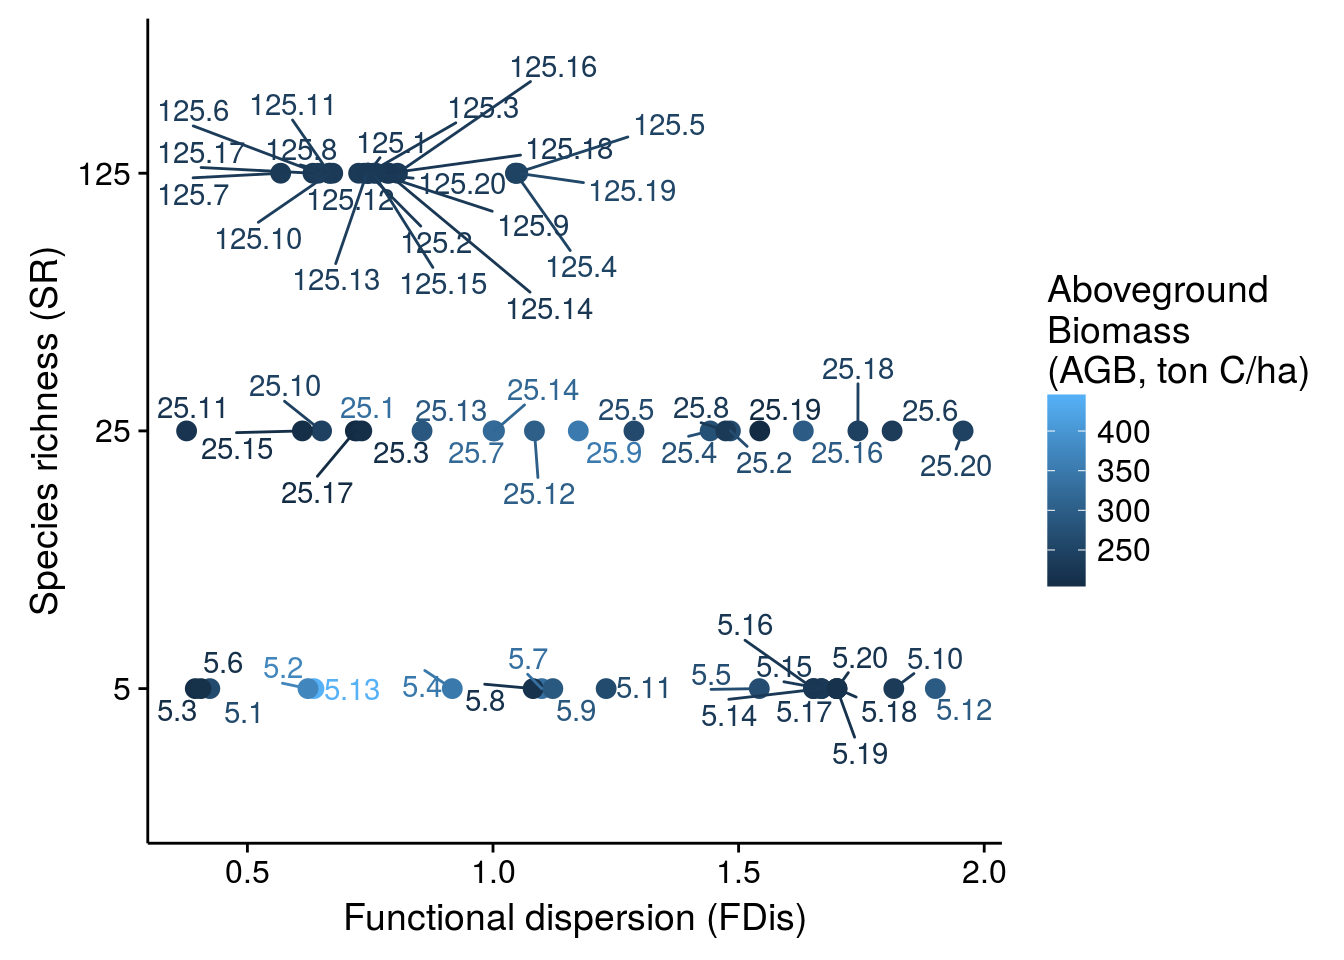
\includegraphics{master-thesis_files/figure-latex/DOE-1.pdf}
\caption{\label{fig:DOE}Experimental design before disturbance. Communities
are implemented along a gradient of species richness (SR) and functional
dispersion (FDis) resulting in a broad range of aboveground biomass
(AGB). FDis was caluclated based on 4 functional traits (leaf mass per
area, wood specific gravity, maximum diameter, maximum height).}
\end{figure}

\subsection{Outputs anlaysis ?}\label{outputs-anlaysis}

\subsubsection{Resistance and resilience
metrics}\label{resistance-and-resilience-metrics}

\subsubsection{Biodiversity
partitioning}\label{biodiversity-partitioning}

\section{Selective logging}\label{selective-logging}

\subsection{Model description}\label{model-description-2}

\subsubsection{Designation}\label{designation}

\subsubsection{Selection}\label{selection}

\subsubsection{Rotten trees}\label{rotten-trees}

\subsubsection{Felling}\label{felling}

\subsubsection{Tracks}\label{tracks}

\subsubsection{Gap damages}\label{gap-damages}

\subsection{Design of experiment}\label{design-of-experiment-1}

\subsection{Outputs analysis ?}\label{outputs-analysis}

\subsubsection{Resistance and resilience
metrics}\label{resistance-and-resilience-metrics-1}

\subsubsection{Biodiversity
partitioning}\label{biodiversity-partitioning-1}

\section{Results}\label{results}

\section{Discussion}\label{discussion}

\bibliography{/home/sylvain/Documents/Bibliography/library.bib}


\end{document}
